%%%% ijcai11.tex

\typeout{IJCAI-13 Instructions for Authors}

% These are the instructions for authors for IJCAI-13.
% They are the same as the ones for IJCAI-11 with superficical wording
%   changes only.

\documentclass{article}
% The file ijcai13.sty is the style file for IJCAI-13 (same as ijcai07.sty).
\usepackage{ijcai13}

% Use the postscript times font!
\usepackage{times}

% the following package is optional:
%\usepackage{latexsym} 

\usepackage{amsthm}
\usepackage{amsmath}
\usepackage{amsfonts}
\usepackage{algpseudocode}
\usepackage{algorithm}
\usepackage{graphicx}

\newtheorem{theorem}{Theorem}
\newtheorem{definition}{Definition}
\newtheorem{corollary}{Corollary}
\newtheorem{lemma}{Lemma}
\newtheorem{proposition}{Proposition}

% Following comment is from ijcai97-submit.tex:
% The preparation of these files was supported by Schlumberger Palo Alto
% Research, AT\&T Bell Laboratories, and Morgan Kaufmann Publishers.
% Shirley Jowell, of Morgan Kaufmann Publishers, and Peter F.
% Patel-Schneider, of AT\&T Bell Laboratories collaborated on their
% preparation.

% These instructions can be modified and used in other conferences as long
% as credit to the authors and supporting agencies is retained, this notice
% is not changed, and further modification or reuse is not restricted.
% Neither Shirley Jowell nor Peter F. Patel-Schneider can be listed as
% contacts for providing assistance without their prior permission.

% To use for other conferences, change references to files and the
% conference appropriate and use other authors, contacts, publishers, and
% organizations.
% Also change the deadline and address for returning papers and the length and
% page charge instructions.
% Put where the files are available in the appropriate places.

\title{IJCAI--13 Formatting Instructions\thanks{These match the formatting instructions of IJCAI-07. The support of IJCAI, Inc. is acknowledged.}}
\author{Francesca Rossi \\
University of Padova\\
Italy \\
pcchair13@ijcai.org}

\begin{document}

\maketitle

\begin{abstract}
  The {\it IJCAI--13 Proceedings} will be printed from electronic
  manuscripts submitted by the authors. The electronic manuscript will
  also be included in the online version of the proceedings. This paper
  provides the style instructions.
\end{abstract}

\section{Introduction}

\section{General Test Game}

A \emph{test game} $G = (A, \mathbb B, p, v, m, t)$ is a 2-player Bayes game
between the tester and the test taker. The tester has a set of potential
problems $A = \{a_1, a_2, \ldots, a_n\}$ to test and the test taker has an
uncertain type (thus Bayes) characterized by $\mathbb B = \{B_1, B_2, \ldots,
B_L\}$. Set $B_l \subseteq A$ is the unsolvable problem set of the $l$-th type
test taker.  Function $p: \mathbb B \rightarrow [0,1]$ characterizes the
probability that a particular type test taker occurs.  The memorize capacity
function $m: \mathbb B \rightarrow \mathbb N$ denotes how many problems a
particular test taker can memorize and the value function $v: \mathbb B
\rightarrow \mathbb R^+$ denotes how much utility the tester gets if that test
taker failed the test (recall that the tester can only fail test takers who
cannot solve all problems and he want to fail as many of them as possible). For
simplicity, we write $p(B_l), m(B_l), v(B_l)$ as $p_l, m_l, v_l$ when the
context is clear.  During the test, $t$ out of $n$ problems will be tested and
a particular test taker will pass the test if all tested problems are either
not in the unsolvable problem set or memorized.  

The game only has two outcomes, pass or fail. The tester gets $0$ utility if a
test taker passes and he gets $v_l$ utility if a type-$l$ test taker fails. On
the type-$l$ test taker's side, he gets $0$ utility if he passes and $-v_l$ if
he fails. From the test taker's perspective, any utility function that has a
higher pass utility than fail utility will give him the same incentive to pass
the test at his best. We define them as $0, -v_l$ specifically for the zero-sum
property of the game.

Our goal is to find the optimal strategy for the tester to maximize his utility
under Stackelberg settings. That is, the tester firstly reveals his strategy
about how $t$ problems are picked to test, then the test taker chooses the best
memorizing strategy. This corresponds to our confidential-free assumption where
test takers know what problems might be tested, their answers, and how likely
they are tested. The only constraint for test takers is that they cannot
memorize too many (greater than $m_l$) problem answers. 

\subsection{General Linear Program (LP) Formulation}

General 2-player Bayes Stackelberg games are NP-hard in terms of game matrix
size so previous work used mixed integer LP (e.g. DOBSS [cite]) to solve them.
We model test games as zero-sum so we can bypass the NP-hardness and use the
following maximin LP to solve our 2-player zero-sum Bayes Stackelberg games in
polynomial time with respect to the game matrix size:

\begin{align}\label{eqn:maximin}
	\max~ &\sum_l p_l V_l \\
	s.t.~ &(\forall l, \forall c_l \in C_l),\nonumber\\
	&~~ \sum_r x_r u^l(r, c_l) \geq V_l\nonumber\\
	&\sum_r x_r = 1\nonumber\\
	&(\forall r \in R) x_r \geq 0\nonumber
\end{align}

where 
\begin{itemize}

 \item $V_l$: utility that the test taker can get from type $l$ test takers

 \item $C_l$: action space of type $l$ test takers, i.e. all combinations of
 problems that they can memorize.

 \item $R$: action space of the tester, i.e. all combinations of problems that
 he can test.
 
 \item $x_r$: probability to test problem set $r$

\end{itemize}

The dual of the above LP is:

\begin{align}\label{eqn:dual-original}
  \min~&U\\
  s.t. &(\forall r) U \geq \sum_{l, c_l} u^l(r, c_l) y_{l, c_l}\nonumber\\
  &(\forall l) \sum_{c_l} y_{l, c_l} = p_l\nonumber\\
  &(\forall l, c_l) y_{l, c_l} \geq 0 \nonumber
\end{align}

which is equivalent to 

\begin{align}\label{eqn:minimax}
  \min~&\max_r(U_r)\\
  s.t. &(\forall r) U_r = \sum_{l, c_l} u^l(r, c_l) y_{l, c_l}\nonumber\\
  &(\forall l) \sum_{c_l} y_{l, c_l} = p_l\nonumber\\
  &(\forall l, c_l) y_{l, c_l} \geq 0\nonumber
\end{align}

The dual LP is as if that all types of test takers share the same goal to lower
the tester's best testing utility ($\max_r (U_r)$ where $U_r$ is the utility of
testing $r$) as much as possible by memorizing problems and revealling their
memorizing strategies $y_{l, c_l}$ to the tester.

However, even if the LPs above are in polynomial size of the game matrix size
(or the action space size), they are exponential to the input of our test
games: the tester's action space is exponential to $t$ (the number of problems
to test) and the type-$l$ test taker's action space is exponential to $m_l$
(the number of problems he can memorize). So those LPs only give us polynomial
algorithms when $m_l, t$ are constant. Our next question is whether the test
game in general can be solved in polynomial time in terms of the input size.

\subsection{Hardness on Test Size}

In order to formally characterize \emph{test game}'s hardness, define

\begin{definition}[\textsc{Optimal Test Strategy} Problem]
Given a test game $G$ and a value $u$, the \textsc{Optimal Test Strategy}
problem is to decide whether the tester has a Stackelberg strategy with at
least $u$ utility.
\end{definition}

It's easy to show

\begin{theorem}\label{thm:test-hardness}
Even if test takers cannot memorize any problems ($m_l = 0$), \textsc{Optimal
Test Strategy} is NP-hard when test size $t$ is non-constant.
\end{theorem}

\begin{proof}
	Reduce a \textsc{Vertex Cover} instance to a \textsc{Optimal Test
	Strategy} instance as follows. Given a graph $G = (V, E)$, construct a
	test game $G'$ with problem set $A = V$.  For each edge $e = \{i, j\}
	\in E$, add one type of test takers $l_e$ whose unsolvable problem set
	$B_{l_e} = e$. Let $p_{l_e} = 1/|E|, v_{l_e} = 1$ and $m_{l_e} = 0$ for
	all $l_e$.  Graph $G$ has a vertex cover of size $k$ if and only if the
	tester has a strategy to test $t = k$ problems and gets $u=1$ utility
	(i.e. all test takers will fail for sure) in test game $G'$.
\end{proof}

\subsection{Hardness on Memorize Capacity}


\begin{theorem}\label{thm:memorize-hardness}
Even if test size is $2$, \textsc{Optimal Test Strategy} is coNP-hard when
memorize capacity is non-constant.
\end{theorem}

\begin{proof}
We reduce \textsc{Independent Set} instances to test games with test size $t=2$
and ask the complementary question: is $u$ the highest utility that the tester
can get. That question has a yes answer if and only if the dual minimax LP
[reference] has a feasible solution with objective at most $u$. For a graph $G
= (V, E)$, let $V$ be our test problem set $A$. Add $L = |E|+|V|+2$ types of
test takers as follows:

\begin{itemize}

\item For each edge $e = (i, j) \in E$, add one type of test takers $l_e$ with
$v_{l_e} = 1$, $B_{l_e} = \{i, j\}$ and $m_{l_e} = 0$.

\item For each vertex $i$, add one type of test takers $l_i$ with $v_{l_i} =
d_G-d(i), B_{l_i} = \{i\}$ and $m_{l_i} = 0$. Here $d_G$ is the maximum vertex
degree in $G$ and $d(i)$ is the degree of vertex $i$. 

\item Add one auxiliary type of test takers $l_\alpha$ with $v_{l_\alpha} =
\alpha \varepsilon, m_{l_\alpha} = 2$ and $B_{l_\alpha} = V$ where $\alpha =
\binom{|V|}{2} - |E|-\binom{k}{2}$ and $\varepsilon \ll 1$. 

\item Finally, add one type of test takers $l_k$ with $v_{l_k} =
\varepsilon, B_{l_k} = V$ and $m_{l_k} = k$.

\end{itemize}

Let all types of test takers occur with uniform probability $p=1/L$.  Then we
show that deciding whether $u = (2 d_G + a\cdot \varepsilon)/L$ is an
upper-bound for the tester's utility, or equivalently whether we can find a
dual solution with objective as low as $u = (2 d_G + a\cdot \varepsilon)/L$ in
our dual minimax LP, is equivalent to finding a size-$k$ independent set in
$G$. Recall that a dual solution is a strategy for test takers to memorize
problems. If no one memorizes, the tester's utility $U_r$ to test a problem set
$r$ is $U_r = (2d_G+a\cdot\varepsilon + \varepsilon) /L$ if $r \notin E$ and
$U_r = (2d_G-1+a\cdot\varepsilon + \varepsilon)/L$ if $r \in E$. To lower the
objective, test takers $l_\alpha, l_k$ should memorize problem sets that bring
the maximum of $U_r$ down.  No matter what the strategy is (as long as they
only memorize unsolvable problems), $\sum_r U_r$ is a constant. And because
$U_r$ for $r \notin E$ is much larger than $U_r$ for $r \in E$ as $\varepsilon
\ll 1$, it's better to only decrease $U_r$ for $r \notin E$. The only way to do
that is to let $l_\alpha$ test takers only memorize pairs of problems that are
not edges and let $l_k$ test takers only memorize size-$k$ indepedent sets of
problems.  If there's a size-$k$ independent set, let $l_k$ test takers
memorize one size-$k$ independent set all the time and let $l_\alpha$ test
takers memorize all pairs of problems that are not covered by that independent
set with uniform probability. That will make $U_r = (2d_G+a\cdot\varepsilon)/L$
for $r \notin E$ and $U_r = (2d_G-1+a\cdot\varepsilon+\varepsilon)/L$ for $r
\in E$.  This is the best they can achieve and this can only be achieved when a
size-$k$ independent set exists in $G$.

\end{proof}

\subsection{Summary on General Test Games}

\begin{theorem}
The \textsc{Optimal Test Strategy} for a \emph{test game} can be computed in
polynomial time when test size and memorize capacity are constant. It's
NP-complete when test size is non-constant and coNP-complete when memorize
capacity is non-constant. Hence it's both NP-hard and coNP-hard when both test
size and memorize capacity are non-constant.
\end{theorem}

\begin{proof}
When test size and memorize capacity are both non-constant, \textsc{Optimal
Test Strategy} is both NP-hard and coNP-hard by Theorem~\ref{thm:test-hardness}
and \ref{thm:memorize-hardness}.  LP~(\ref{eqn:maximin}) shows that
\textsc{Optimal Test Strategy} can be computed in polynomial time when test
size and memorize capacity are constant.  When memorize capacity is constant or
test size is constant, either the primal LP~(\ref{eqn:maximin}) or the dual
LP~(\ref{eqn:minimax}) has constant number of constraint. Such LP has a
polynomial size optimal solution even if the number of variables is
exponential. That optimal solution's feasibility and objective can be checked
in polynomial time. Therefore \textsc{Optimal Test Strategy} is in NP when
memorize capacity is constant and it is in coNP when test size is constant.
Hence they are NP-complete and coNP-complete respectively by
Theorem~\ref{thm:test-hardness} and \ref{thm:memorize-hardness}. 
\end{proof}

[HARDNESS TABLE]

\section{One-Problem Test Game}

We showed the hardness of test games when either one of test size or memorize
capacity is non-constant. When the test size is non-constant, there is little
we can improve because it is NP-hard even if the memorize capacity is zero.
When the memorize capacity is non-constant, our proof for
Theorem~\ref{thm:memorize-hardness} only showed that NP-hardness for testing 2
problems. Therefore an efficient algorithm to compute optimal one-problem test
may exist. 

We firstly investigated such tests by conducting experiments using
LP~(\ref{eqn:maximin}). Surprisingly, no matter how input varies, the strategy we get
always has the following format: among a subset $T$ of problems $A$, test any
one of them with uniform probability. That is counter-intuitive as some
problems in $T$ seem to be obviously more superior than others so intuitively they should
be tested with more probability. For example, when $n$ problems can be sorted
by difficulty, a test taker who can solve a harder problem can always solve an
easier problem. In that case, it seems that the hardest problem should be
tested strictly more likely than the second hardest problem. But in most cases,
the optimal strategy will test one of them with equal probability.

[EXAMPLE TABLE]

Nevertheless, such uniform test property looks to be a good news for us to find
an efficient algorithm for solving one-problem test. Inspired by that
uniform test property, we present an algorithm to compute optimal strategies
and use it to prove uniform test property consequently.

\begin{algorithm}\label{alg:one-problem}
\caption{Compute the optimal one-problem test strategy with an acceptable
objective error $\epsilon$ (for binary search)}
\begin{algorithmic}[1]
\Function{OptimalOneProblemTest}{$A, \mathbb B, m, v, p$}
	\ForAll{$a \in A$} \Comment{Utility without memorizing}
		\State $U^0_a \gets \sum_{B_l \ni a} v_l p_l$ 
	\EndFor
	\State $U_{lower} \gets 0, ~U_{upper} \gets \max_{a \in A} U^0_a$
	\While{$U_{upper}-U_{lower} > \epsilon$}\Comment{Binary search}
		\State $U \gets (U_{upper}+U_{lower})/2$ \Comment{Objective utility}
		\State $V \gets \{s\} \cup \mathbb B \cup A \cup \{t\}$ \Comment{Vertex set}
		\State $E \gets \emptyset$ \Comment{Initialize edge set}
		\ForAll{$a \in A$}
			\If{$U^0_a > U$}
				\State $E \gets E \cup \{(a, t)\}$
				\State $c_{(a, t)} \gets U^0_a-U$ \Comment{Edge capacity}
			\EndIf
		\EndFor
		\ForAll{$B_l \in \mathbb B$} 
			\State $E \gets E \cup \{B_l\} \times B_l$ %\Comment{Edges between $\mathbb B$ and $A$}
			\State $c_{\{B_l\} \times B_l} \gets p_l v_l$ 
			\State $E \gets E \cup \{(s, B_l)\}$ %\Comment{Edges between $\{s\}$ and $\mathbb B$}
			\State $c_{(s, B_l)} \gets p_l m_l v_l$
		\EndFor
		\State $f \gets \Call{MaxFlow}{G = (V, E), c}$
		\If{$f$ saturates all edges in $A \times \{t\}$}
			\State $U_{upper} \gets U$
		\Else
			\State $U_{lower} \gets U$
		\EndIf
	\EndWhile
	\State $T \gets \{a ~|~ U^0_a \geq U\}$
	\State $Q \gets $ all $B_l$ such that $(s, B_l)$ is not saturated in $f$
	\State $G(B_l) \gets c_{(s, B_l)}-f_{(s, B_l)}$ \Comment{Potential flow} \label{line:first-potential}
	\While{$Q$ has an unmarked element}
		\State $B_l \gets $ get and mark an unmarked element from $Q$
		\ForAll{$a \in B_l$ and $(B_l, a)$ is not saturated in $f$}
			\State $T \gets T \backslash \{a\}$\label{line:delete-a}
			\ForAll {$B_{l'} \ni a $ and $ f_{(B_{l'},a)}>0$}
				\State $G(B_{l'}) \gets \min(f_{(B_{l'},a)}, \frac{G(B_l)}{|B_l|L})$\label{line:second-potential}
				\State Push $B_{l'}$ into $Q$
			\EndFor
		\EndFor
	\EndWhile
	\State \Return{Strategy that test $T$ uniformly}
\EndFunction
\end{algorithmic}
\end{algorithm}

The algorithm consists of two parts. It firstly uses binary search and max flow
to determine the optimal tester's utility $U$.  This part corresponds to the following
LP formulation (let $U^0_a$ be the utility of testing $a$ without memorizing as we defined
in Algorithm~\ref{alg:one-problem}):
\begin{align}\label{eqn:one-problem}
	\min~ &U\\
	s.t.~ &(\forall a \in A)~ U \geq U^0_a - \sum_{B_l \ni a} v_l z_{l, a}\nonumber\\
	&(\forall l)~ \sum_{a \in B_l} z_{l, a} \leq m_l p_l\nonumber\\
	&(\forall l, a)~ 0 \leq z_{l, a} \leq p_l\nonumber
\end{align}
This LP modifies LP~(\ref{eqn:dual-original}) by:
\begin{enumerate}
	\item Change joint probability $y_{l, c_l}$ to marginal probability
	$z_{l, a}$ of memorizing one problem $a$.  We did this modification
	because marginal probability is more meaningful for one-problem test
	and we can always restore a joint probability from a marginal
	probability[reference].
	\item Relax equality $\sum_{a \in A} z_{l, a} = m_l p_l$ to inequality $\sum_{a \in A} \leq m_l p_l$. 
	We can do this because $v_l \geq 0$ (thus $u^l, V_l \geq 0$) and this modification
	is essentially adding $V_l \geq 0$ to the primal LP~(\ref{eqn:maximin}).
\end{enumerate}
With a given $U$, we use max flow to check its feasibility. Intuitively, a $U$
is feasible if and only if there is a strategy $z_{l, a}$ such that for every
$a$ where $U^0_a > U$, that strategy $z_{l, a}$ decrease it down to $U$. This
is achievable if and only if the max flow can saturate all edges from $A$ to
$t$. The max flow $f$ can also compute that strategy by setting $z_{l, a} =
f_{(B_l, a)}/v_l$.

The second part of the algorithm is to compute the test strategy (the optimal
primal solution) from the memorize strategy (the optimal dual solution) we
computed in the first part by max flow. We prove that our test strategy is
optimal by complementrary slackness theorem, which in our context is
essentially: 1) the tester only tests problems (non-zero primal variables)
that gives him best utility (tight dual constraints); 2) the test taker only
memorizes problems (non-zero dual variables) that gives him best utility
(tight primal constraints).\footnote{This is essentially saying that in a
zero-sum game, a minimax, or maximin state is reached, if and only if the Nash
equilibrium is reached.} We will need two more lemmas as follows to use the
complementary slackness theorem.

\begin{lemma}\label{lemma:best-response}
Let $z_{l,a} = f_{(B_l, a)}/v_l$ be the dual solution computed by max flow and
$T$ be the final subset that Algorithm~\ref{alg:one-problem} returns. Then for
each type of test takers $B_l$, either $\sum_{a \in B_l} z_{l,a} = m_l p_l$
(they memorize a subset of $T$ all the time) or $\forall a \in B_l \cap T,
z_{l, a} = p_l$ (they memorize unsolvable problems in $T$ all the time so they
will pass the test for sure).
\end{lemma}
\begin{proof}
If there is a $B_l$ such that $\sum_{a \in B_l} z_{l,a} < m_l p_l$, either 
$f_{s, B_l}$ is not saturated or there is an $a \in B_l$ with $f_{(B_l, a)} >
0$ that is deleted from $T$ later on line~\ref{line:delete-a} of
Algorithm~\ref{alg:one-problem}. In any case, $B_l$ will be pushed into $Q$ and
all problems in $B_l$ that does not satisfy $z_{l,a} = p_l$ will be deleted
from $T$. Hence $\forall a \in B_l \cap T, z_{l, a} = p_l$ must hold.
\end{proof}

\begin{lemma}\label{lemma:non-empty}
$T$ returned by Algorithm~\ref{alg:one-problem} is non-empty.
\end{lemma}
\begin{proof}
$T$ is non-empty before we delete problems from $T$ on
line~\ref{line:delete-a} of Algorithm~\ref{alg:one-problem}.  Denote that
initial $T$ as $T_0$.  If all problems in $T_0$ are deleted, then for every $a$
in $T_0$ there is a $B_l$ that is in $Q$ and $f_{(B_l, a)}$ is not saturated.
Note that for every $B_l$ in $Q$, it has a positive potential flow $G(B_l)$
that can additionally flow out of vertex $B_l$, either because $(s, B_l)$ is
not saturated (on line \ref{line:first-potential}) or because there is a
positive flow $(B_l, a)$ that can be reduced (on line
\ref{line:second-potential}). This means that we can bring $U$ down by sending
these potential flow to every vertex in $T_0$, a contradiction to that
$U$ is minimized.
\end{proof}

\begin{theorem}
Uniformly testing $T$ returned by Algorithm~\ref{alg:one-problem} is optimal.
\end{theorem}
\begin{proof}
First of all, $T$ is non-empty by Lemma~\ref{lemma:non-empty} so we can test
$T$ uniformly. Then since the max flow makes $U_a$ (the utility to test a
problem $a$) decrease to $U$ if $U^0_a > U$ and we only pick $T$ from problems
that $U^0_a > U$, every problem that we might test gives the tester best
utility. That is the first condition for the complementary slackness theorem.
Finally, Lemma~\ref{lemma:best-response} show that one type of test takers
either pass the test for sure or memorize a subset in $T$ all the time which is
optimal for uniform test, the second condition of complementary slackness
theorem holds.
\end{proof}


\section{Experiment}

In this section, we conduct experiments to see how different algorithms scale
on test games. 

EXPERIMENTS FOR MULTI-PROBLEM TEST?

For one-problem test, our original LP~(\ref{eqn:maximin}) is exponential to the
memorize capacity so we only compare modified LP~(\ref{eqn:one-problem}) and
max flow based Algorithm~\ref{alg:one-problem}.  During each experiment, we
specify four parameters $n, L, m_{max}, b_{max}$, the number of problems, the
number of test taker types, the maximum memorize capacity and the maximum size
of $B_l$. Given those parameters, a test game instance is generated as follows:
for each $1 \leq l \leq L$, generate $m_l$ uniformly from $1$ to $m_{max}$,
generate $|B_l|$ uniformly from $m_l$ to $b_{max}$, generate $B_l$ by selecting
$|B_l|$ elements from $A$ uniformly and generate $w_l = v_l p_l$ (weight of
type-$l$) from $[0,1]$ uniformly. Here we only generate $w_l$ because $v_l$ and
$p_l$ always appear together as $v_l p_l$.

For each parameter setting, we generate $5$ test game instances and compute
the average running time for each algorithm. During each run, we set timeout to
be 5 seconds. For the LP, we ran it on glpk and cplex.  For the max flow, we
tried both Edmonds-Karp and Push-Relabel implementation in C++ boost library.

\begin{figure}
	\caption{Average running time for different one-problem test algorithms
	over the number of problems $n$. For each $n$, we set the other three
	parameters $L = n, m_{max} = \lfloor \sqrt{n} \rfloor$ and $b_{max} =
	2m_{max}$ (see Table~\ref{tab:settings}).}
	\label{fig:benchmark}
	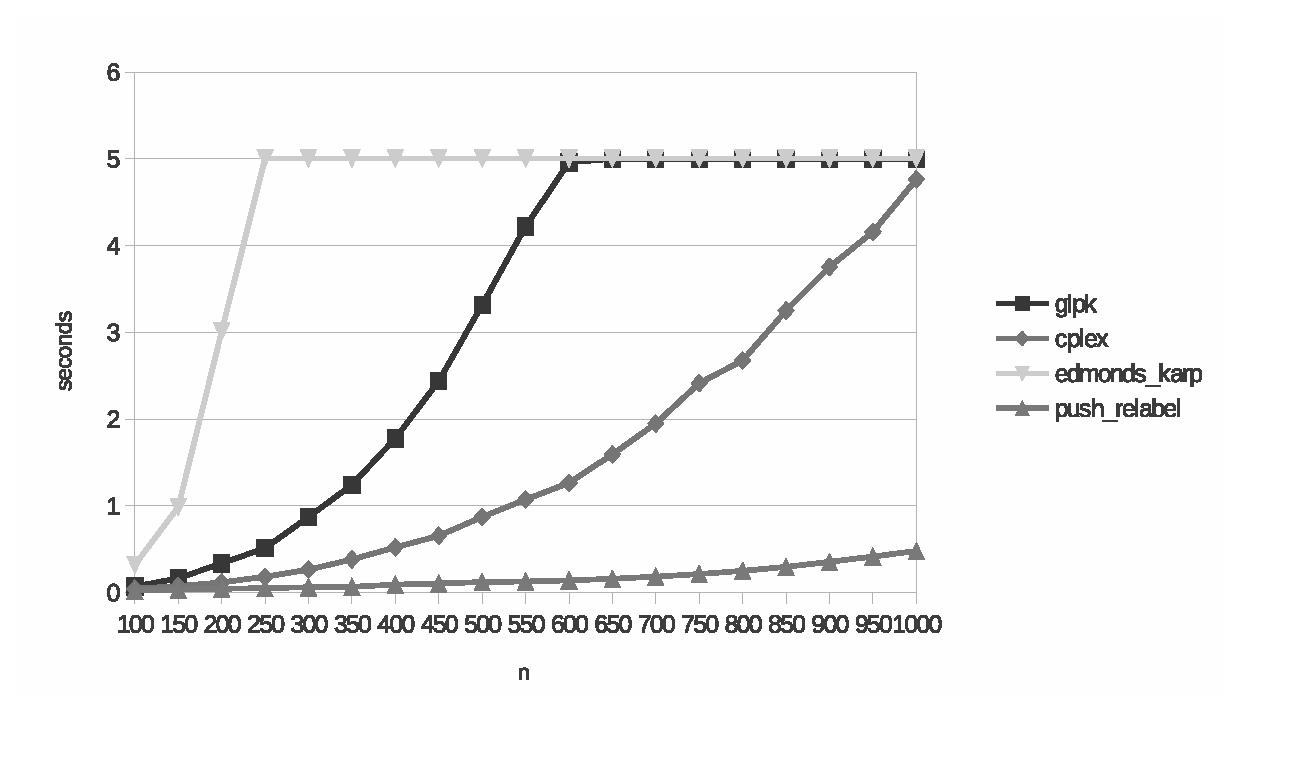
\includegraphics[trim=5mm 0 15mm 0, clip, width=\linewidth]{benchmark}
\end{figure}

In our benchmark, we increase $n$ and set the remaining three parameters $L,
m_{max}, b_{max}$ as following: $L = n, m_{max} = \lfloor \sqrt{n} \rfloor$ and
$b_{max} = 2m_{max}$. Note that our $L, b_{max}$ are quite small (they can be
as large as $b_{max} = n/2, L = \binom{n}{b_{max}})$. That's becuase for large $L,
b_{max}$, our uniform random input will almost always make the trivial strategy
to uniformly test among all $n$ problems optimal. So we make them small to
avoid such trivial solutions. The realized parameter settings are shown in
Table~\ref{tab:settings} (we show them in the step of 50 for the sake of
space). The benchmark is shown in Figure~\ref{fig:benchmark}.

\begin{table}
	\caption{Parameter settings for the benchmark}\label{tab:settings}
	\begin{center}
	\begin{tabular}{ r r r r }
		$n$&$L$&$m_{max}$&$b_{max}$\\
		\hline\\
		100&100&10&20\\
%		150&150&12&24\\
		200&200&14&28\\ 
%		250&250&15&30\\
		300&300&17&34\\
%		350&350&18&36\\
		400&400&20&40\\
%		450&450&21&42\\
		500&500&22&44\\
%		550&550&23&46\\
		600&600&24&48\\
%		650&650&25&50\\
		700&700&26&52\\
%		750&750&27&54\\
		800&800&28&56\\
%		850&850&29&58\\
		900&900&30&60\\
%		950&950&30&60\\
		1000&1000&31&62
	\end{tabular}
	\end{center}
\end{table}


\section{Conclusion}

\section*{Acknowledgments}

The preparation of these instructions and the \LaTeX{} and Bib\TeX{}
files that implement them was supported by Schlumberger Palo Alto
Research, AT\&T Bell Laboratories, and Morgan Kaufmann Publishers.
Preparation of the Microsoft Word file was supported by IJCAI.  An
early version of this document was created by Shirley Jowell and Peter
F. Patel-Schneider.  It was subsequently modified by Jennifer
Ballentine and Thomas Dean, Bernhard Nebel, and Daniel Pagenstecher.
These instructions are the same as the ones for IJCAI--05, prepared by
Kurt Steinkraus, Massachusetts Institute of Technology, Computer
Science and Artificial Intelligence Lab.

\appendix

\section{\LaTeX{} and Word Style Files}\label{stylefiles}

The \LaTeX{} and Word style files are available on the IJCAI--13
website, {\tt http://www.ijcai-13.org/}.
These style files implement the formatting instructions in this
document.

The \LaTeX{} files are {\tt ijcai13.sty} and {\tt ijcai13.tex}, and
the Bib\TeX{} files are {\tt named.bst} and {\tt ijcai13.bib}. The
\LaTeX{} style file is for version 2e of \LaTeX{}, and the Bib\TeX{}
style file is for version 0.99c of Bib\TeX{} ({\em not} version
0.98i). The {\tt ijcai13.sty} file is the same as the {\tt
ijcai07.sty} file used for IJCAI--07.

The Microsoft Word style file consists of a single file, {\tt
ijcai13.doc}. This template is the same as the one used for
IJCAI--07.

These Microsoft Word and \LaTeX{} files contain the source of the
present document and may serve as a formatting sample.  

Further information on using these styles for the preparation of
papers for IJCAI--13 can be obtained by contacting {\tt
pcchair13@ijcai.org}.

%% The file named.bst is a bibliography style file for BibTeX 0.99c
\bibliographystyle{named}
\bibliography{ijcai13}

\end{document}

